\begin{figure}[h]
    \centering
    \begin{subfigure}[b]{0.45\textwidth}
        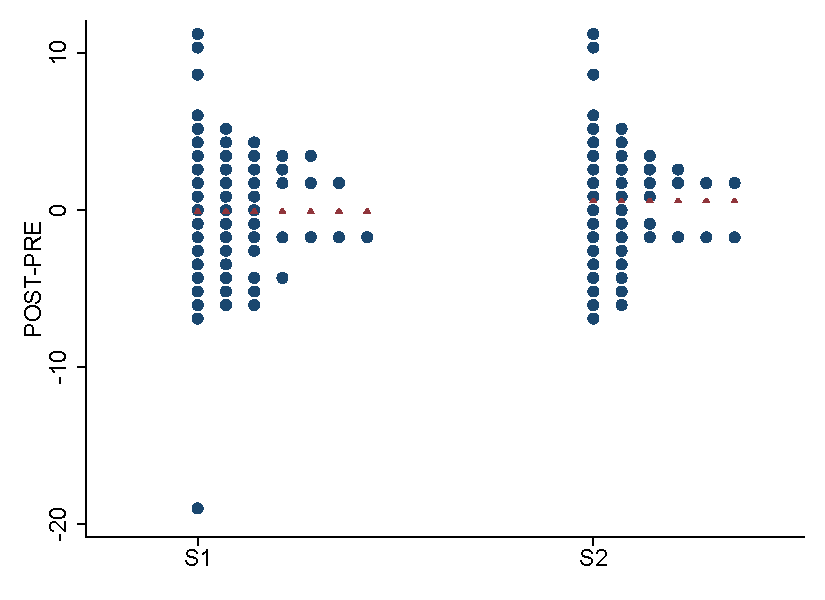
\includegraphics[width=\textwidth]{Figures/JO_distribution.pdf}
        \caption{\cite{jones2004leaders}'s leaders}
        \label{fig:JO}
    \end{subfigure}
    \\ %add desired spacing between images, e. g. ~, \quad, \qquad, \hfill etc. 
      %(or a blank line to force the subfigure onto a new line)
    \begin{subfigure}[b]{0.45\textwidth}
        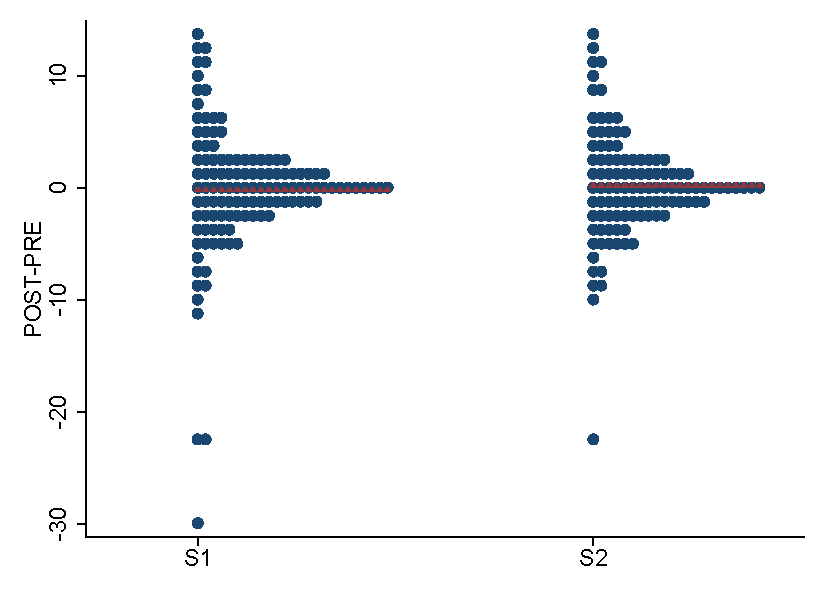
\includegraphics[width=\textwidth]{Figures/Besley_distribution.pdf}
        \caption{\cite{besley2011educated}'s leaders}
        \label{fig:Besley}
    \end{subfigure}
    %~ %add desired spacing between images, e. g. ~, \quad, \qquad, \hfill etc. 
    %(or a blank line to force the subfigure onto a new line)
    \\
    \begin{subfigure}[b]{0.45\textwidth}
        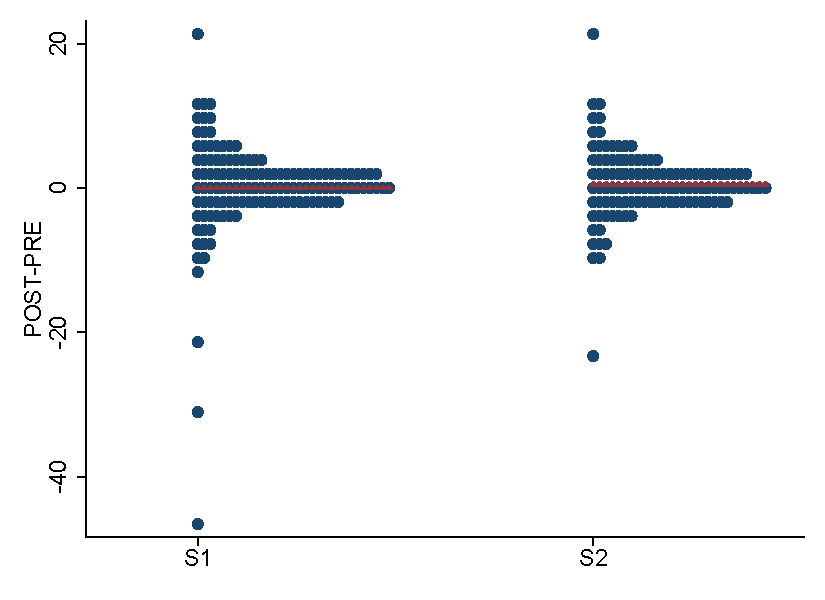
\includegraphics[width=\textwidth]{Figures/Own_distribution.pdf}
        \caption{Our leaders}
        \label{fig:Own}
    \end{subfigure}
    \caption{Distribution of $\overline{POST}_z-\overline{PRE}_z$.}\label{fig:distribution}
    \medskip % induce some separation between caption and explanatory material
    \begin{minipage}{0.9\textwidth} % choose width suitably
    	{\footnotesize  Notes: the values are grouped together vertically and plotted as blue points separated horizontally. The red triangles indicate the mean in each sample. The $PRE_z$ and $POST_z$ dummies are estimated via GLS allowing for country-specific heteroskedasticity and panel-specific AR(1) autocorrelation.\par}
    \end{minipage}
\end{figure}
